\documentclass[border=10pt]{standalone}
\usepackage[svgnames]{xcolor}
\usepackage{amsmath}
\usepackage{pgfplots}
\pgfplotsset{compat=newest}
\usepackage[sfdefault]{FiraSans}
\usepackage{FiraMono}
\renewcommand*\familydefault{\sfdefault}
\begin{document}
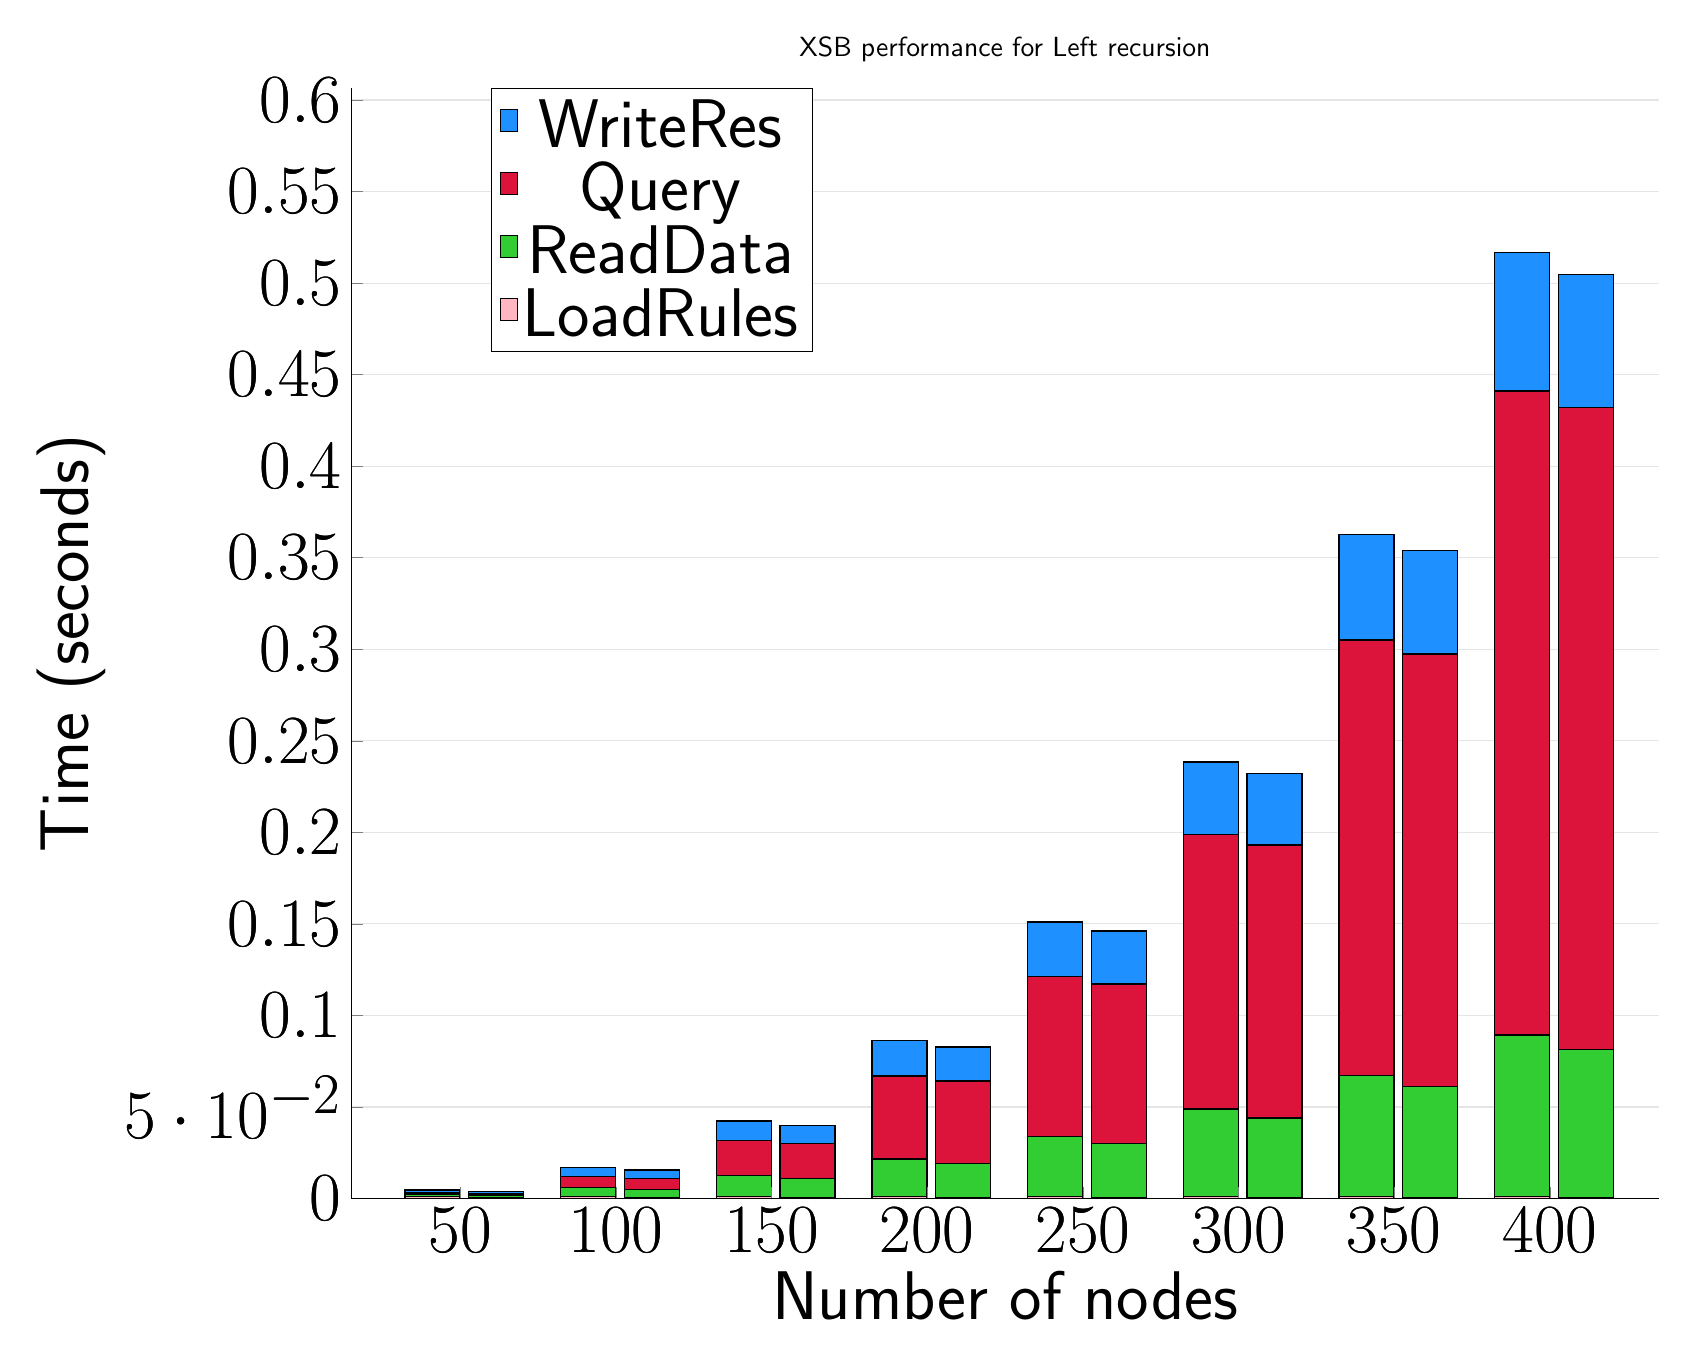
\begin{tikzpicture}
	\begin{axis}[
			ybar stacked,
			title={XSB performance for Left recursion},
			bar shift=-10pt,
			width=1.5\textwidth,
			bar width=0.7cm,
			ymajorgrids, tick align=inside,
			major grid style={draw=gray!20},
			xtick=data,
			ymin=0, ymax=0.6066430044174194,
			axis x line*=bottom,
			axis y line*=left,
			enlarge x limits=0.1,
			legend style={
					at={(0.23, 1)},
					anchor=north,
					legend columns=1,
					font=\Huge,
				},
			ylabel={Time (seconds)},
			xlabel={Number of nodes},
			label style={font=\Huge},
			tick label style={font=\Huge},
		]
		\addlegendimage{fill=DodgerBlue, draw=black, line width=0.2pt}
		\addlegendentry{WriteRes}
		\addlegendimage{fill=Crimson, draw=black, line width=0.2pt}
		\addlegendentry{Query}
		\addlegendimage{fill=LimeGreen, draw=black, line width=0.2pt}
		\addlegendentry{ReadData}
		\addlegendimage{fill=LightPink, draw=black, line width=0.2pt}
		\addlegendentry{LoadRules}
		\addplot +[fill=LightPink, draw=black, line width=0.5pt] coordinates {
				(50, 0.0010438203811645509)
				(100, 0.001057696342468262)
				(150, 0.0010444402694702141)
				(200, 0.0010344505310058599)
				(250, 0.001076650619506837)
				(300, 0.0010499000549316418)
				(350, 0.001066899299621582)
				(400, 0.00106961727142334)
			};
		\addplot +[fill=LimeGreen, draw=black, line width=0.5pt] coordinates {
				(50, 0.001464271545410156)
				(100, 0.005079793930053712)
				(150, 0.01139140129089355)
				(200, 0.02056140899658204)
				(250, 0.03284051418304444)
				(300, 0.0478470802307129)
				(350, 0.06610300540924073)
				(400, 0.0881951093673706)
			};
		\addplot +[fill=Crimson, draw=black, line width=0.5pt] coordinates {
				(50, 0.0007915019989013672)
				(100, 0.005823993682861328)
				(150, 0.019289684295654305)
				(200, 0.04530677795410156)
				(250, 0.08730089664459227)
				(300, 0.14992632865905747)
				(350, 0.237977385520935)
				(400, 0.3518773317337036)
			};
		\addplot +[fill=DodgerBlue, draw=black, line width=0.5pt] coordinates {
				(50, 0.0013949871063232428)
				(100, 0.005062675476074202)
				(150, 0.01057443618774413)
				(200, 0.019316053390502942)
				(250, 0.02986266613006583)
				(300, 0.03962666988372811)
				(350, 0.0575848579406739)
				(400, 0.07544789314270021)
			};
	\end{axis}
	\begin{axis}[
			ybar stacked,
			bar shift=13pt,
			width=1.5\textwidth,
			bar width=0.7cm,
			ymajorgrids, tick align=inside,
			major grid style={draw=none},
			xtick=data,
			ymin=0, ymax=0.6066430044174194,
			axis x line*=none,
			axis y line*=none,
			enlarge x limits=0.1,
			label style={font=\Huge},
			tick label style={font=\Huge},
		]
		\addplot +[fill=LightPink, draw=black, line width=0.5pt] coordinates {
				(50, 0.0006081000000000005)
				(100, 0.0006204000000000001)
				(150, 0.0006104000000000002)
				(200, 0.0006000000000000001)
				(250, 0.0006129000000000004)
				(300, 0.0006057999999999993)
				(350, 0.0006081999999999999)
				(400, 0.0006078000000000006)
			};
		\addplot +[fill=LimeGreen, draw=black, line width=0.5pt] coordinates {
				(50, 0.0011595999999999998)
				(100, 0.004443000000000001)
				(150, 0.0102165)
				(200, 0.0185578)
				(250, 0.029586499999999995)
				(300, 0.04339439999999999)
				(350, 0.060472399999999996)
				(400, 0.0808092)
			};
		\addplot +[fill=Crimson, draw=black, line width=0.5pt] coordinates {
				(50, 0.0007838000000000001)
				(100, 0.0057867)
				(150, 0.019170200000000002)
				(200, 0.04508739999999999)
				(250, 0.0869516)
				(300, 0.1490527)
				(350, 0.2363366)
				(400, 0.3505347)
			};
		\addplot +[fill=DodgerBlue, draw=black, line width=0.5pt] coordinates {
				(50, 0.0011656)
				(100, 0.004712200000000001)
				(150, 0.0099514)
				(200, 0.018474)
				(250, 0.029002400000000005)
				(300, 0.0389818)
				(350, 0.05641630000000001)
				(400, 0.0727807)
			};
	\end{axis}
\end{tikzpicture}

\end{document}
